\documentclass[12pt]{report}
\usepackage[utf8]{inputenc}
\usepackage{graphicx}
\graphicspath{ {Pictures/} }
\usepackage{indentfirst}
\usepackage{setspace}
\usepackage{scrextend}
\usepackage{geometry}
\usepackage{amsmath}
\usepackage{amsfonts}
\usepackage{fancyhdr}
\usepackage{relsize}
\usepackage{amsthm}
\usepackage{amssymb}
\usepackage{tikz}
\usepackage{imakeidx}
\usepackage{mathrsfs} 
\usepackage[english]{babel}
\usepackage{accents}
\newcommand{\qeq}{\accentset{?}{=}}
\setstretch{1.25}
\pagestyle{fancy}
\fancyhf{}
\rhead{Page \thepage}
\lhead{Approximation Algorithms}

 \geometry{
 a4paper,
 total={170mm,257mm},
 left=20mm,
 top=20mm,
 }

\title{
{Approximation Algorithms Hand Book}\\

{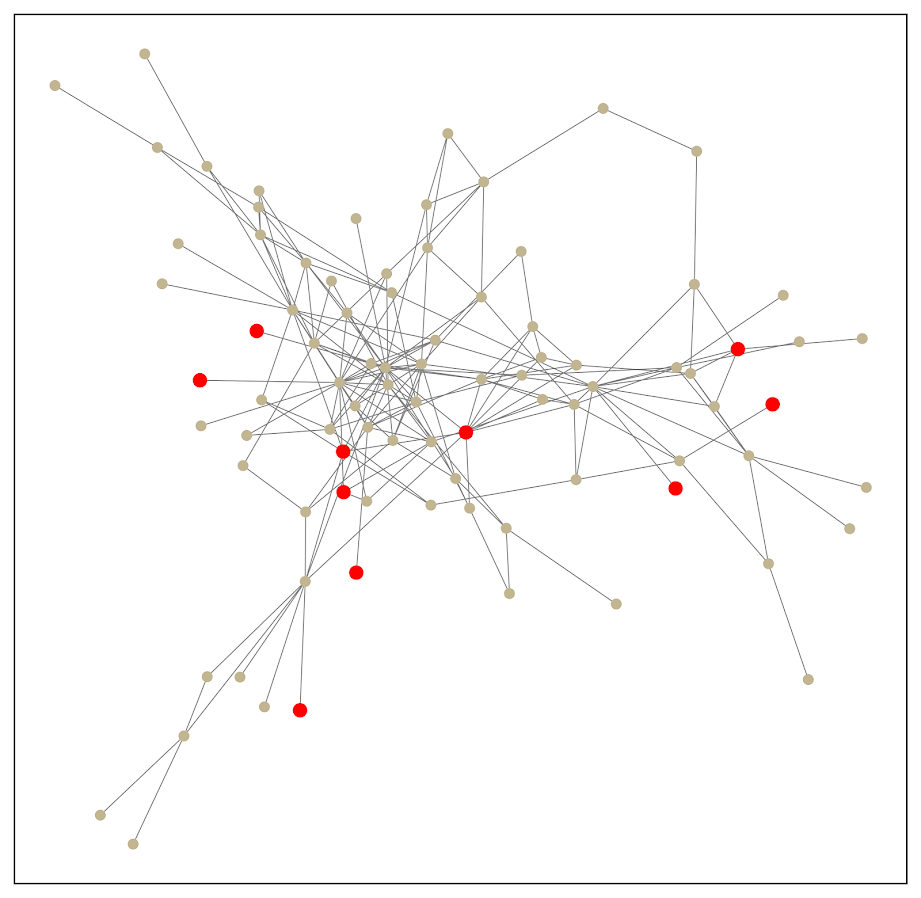
\includegraphics[width=12cm, height=12cm]{hmpg.jpg}}
}
\author{Shreya Patil\\IIIT-H}
\date{29 November 2021}

\setlength\parindent{0pt}
\makeindex

\begin{document}
\maketitle


\chapter{Need for Approximation Algorithms}
We start off by understanding the need for Approximation Algorithms. Having studied dynamic programming, you are familiar with the trade-off that we often make between the time and the space required to solve a problem. This is just an example of trade-off between resources that you will see throughout your journey in Computer science. Approximation Algorithms make such a trade-off between time required to solve a problem and the precision of the solution. In this chapter we will try to understand why this trade-off is necessary, and on which problems it is beneficial. \\

To do this we must first classify problems based on their hardness (There is no point to finding an approximate solution to an easy problem) The hardness would be a measure of the resources consumed by a theoretical computer to solve this problem.\\ 
We can consider this computer to be a Deterministic Turing Machine, but, it is usually preferred to think of it as a Random Access Machine (RAM) which is a machine of your design, that can perform certain tasks such as moving 2 numbers in memory(provided memory is finite), adding 2 small numbers, and other such operations in constant non-zero time. This machine is defined such that it is equal in power to a Turing machine or your personal computer(provided your PC is not a quantum computer). \\
Regardless of how you choose to design this computer, it must have the following restrictions to make the model equivalent to an actual computing device :
\begin{itemize}
  \item It takes non-zero time to retrieve data from far away locations. i.e. The computer has a finite Random Access Memory
  \item A finite machine can only store finite amount of information.
  \item A finite amount of code only exerts finite amount of control.
\end{itemize}

Using this, we can start classifying our problem statements by their hardness.

\subsection*{Class P}
The class P consists of all problems that can be solved in polynomial order time. These are problems that are considered 'easy'.\\
Remember the phrase 'Polynomial is the new constant'.\\
Just as we ignored constant factors in time complexities while studying asymptotic growth, we will ignore polynomially time reductions between solutions. i.e. if a polynomial time reduction exists from problem A to problem B, problem B is atleast as hard as problem A. 

\subsection*{Class NP}
NP stands for Non-deterministic polynomial time, and the class NP contains all problems that can be verified in polynomial time. This means that given a solution to a problem, can you(a deterministic Turing machine) verify the correctness of this solution ? If yes, the problem is in NP. \\
This, of course contains the class P since any problem that can be solved in polynomial time can also be verified in polynomial time, simply by solving it.

\subsection*{Class NP-Hard}
The problems in this class can be defined as at least as hard as the hardest problems in NP. The phrase atleast as hard implies a polynomial time reduction. This contains a lot of problems that are of interest to us in this book, however it also contains some problems that are too hard to verify. Hence, we need a narrower class of problems to work with.

\subsection*{Class NP-Complete}
The very definition of NP-Hard implies that there is some intersection between NP-hard and NP. This intersection is called NP-Complete. These are problems that are too hard to solve but are not beyond hope for approximation algorithms as their solutions can be compared and verified. \\
\pagebreak
\begin{figure}[h]
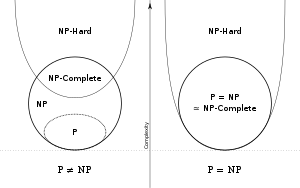
\includegraphics[width=11cm, height=7cm]{np.jpg}
\centering
\end{figure}\\
The above figure shows the set diagrams of the classes of problems. The figure on the right refers to the case where $P=NP$ where any problem that can be verified in polynomial time can be solved in polynomial time. The problem of $P\qeq NP$ is one of the most researched yet unsolved problems in Mathematics and Computer Science. \\
In fact, if $P=NP$ you might as well stop reading this book as all the problems in this book have a polynomial time optimal solution. 
%%%%%%%%%%%%%%%%%%%%%%%%%%%%%%%%%%%%%%%%%%%%%%%%%%%%%%%%%%%%%%%%%%%%%%%%%%%%%%%%%%%%%%%%%%%

\chapter{Greedy Algorithms}
We start off with a familiar paradigm of algorithm design, and with the problem that sparked the research in modern complexity theory and approximation algorithms in - The Set Cover Problem.\\

Before we get to the problem, we start by asking what a greedy approximation algorithm looks like. Is it much different from the greedy algorithms that we have studied previously ? The answer is NO.\\
General Steps in designing greedy approximation Algorithms :
\begin{enumerate}
  \item Choose the right Parameter for the greedy choice, sort the input accordingly.
  \item Make the greedy choice, and add it to the solution
  \item Repeat step2
\end{enumerate}
The only difference in greedy Approximation algorithms is that we do not know what the optimum greedy choice is at each step. instead, we make a 'approximately optimum' choice.

\subsection*{Set Cover Problem}
The problem asks - Given a Set $S$ of cardinality $n$, a subsets of $P(S)$, what subsets must we choose to cover the set S, and minimize the number of chosen subsets.
\begin{align*}
& S = \{a, b, c, d, e\} \\
& S_1 = \{a, c, d\}   \\
& S_2 = \{d, e\}     \\
& S_3 = \{a, b, c, d\}\\
\end{align*}
There are two possible set covers $\{S1, S2\}$ and $\{S2, S3\}$, both are minimal \\

\emph{The Greedy Choice} : In designing a greedy algorithm, this is where the algorithmist must come up with a clever way to make a greedy choice. However, in this problem a intuitive option presents itself. And as it turns out, this is the best possible greedy choice. \\
We define a quantity $\rho(S_i)$ as :
\begin{align*}
\rho(S_i) = |S_i - X| 
\end{align*}
Here X is the set of elements already added to the proposed solution.
$\rho(S_i)$ can be seen as a measure of costs of adding the set $S_i$ given $X$.\\

\textbf{Analysis}\\
It is easy too see that this algorithm is not optimal. Here's a counter-example. 
\begin{align*}
& S = \{a, b, c, d, e, f, g, h\} \\
& S_1 = \{a, b, c, d\}  \\
& S_2 = \{e, f, g, h\}     \\
& S_3 = \{a, b, d, e, f\}  \\
& S_4 = \{c, d\}  \\  
\end{align*}
Here we can see that the optimal solution is $\{S_1, S_2\}$ with 2 elements, and yet the algorithm chooses $\{S_3, S_2, S_4\}$ with 3 elements. Though this doesn't mean that the algorithm is a poor Approximation Algorithm.
Let $OPT$ be the cost of optimal solution. Say $(k-1)$ is the number of elements not covered after $t$ greedy choices. \\
Note that OPT covers more than(or equal to) $n_t$ elements in S. Hence, by the pigeon hole principle, atleast one eof the remaining sets must have $n_t/OPT$ elements.
\begin{align*}
\therefore \quad &n_{t+1} \leq n_t - \frac{n_t}{OPT} \\
\Rightarrow \quad &n_t = ne^{\frac{t}{OPT}} \\
\Rightarrow \quad &t = OPT \cdot log(n)
\end{align*}
We have just shown that the greedy algorithm gives a $O(log(n))$ approximation to optimal solution of the set cover problem.In fact, no polynomial time algorithm can give a better approximation unless $P = NP$.
\pagebreak
\subsection*{Vertex Cover Problem}
The vertex cover is another well known problem that is NP-Complete. \\ 
We will not explicitly solve this problem, since we have already SOLVED it! The goal of this section however is to demonstrate the concept of polynomial time reductions mentioned in chapter 1.\\
The problem statement is as follows :\\
Given a Graph$(G)$, find a sub-set$(S)$ of the vertex set of the graph such that for every edge in the graph, at least one of the vertices of the edge is in $S$.
\begin{align*}
\forall_{uv \in E} \quad u \in V \quad OR \quad v \in V
\end{align*}
Here $E$, $V$ have their usual meaning.\\
If you look carefully, you will notice that this problem has something in common with the Set Cover problem(Not just the Name). \\
\begin{figure}[h]
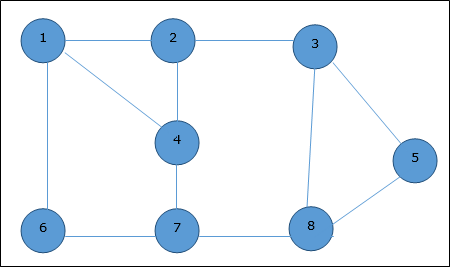
\includegraphics[width=8cm, height=4.8cm]{v_cover.jpg}
\centering
\end{figure}
In the above figure, notice that if we select the vertices 7 and 6, we need not select the vertex 6, as all the edges of 6 have already been covered, furthermore, the benefit of choosing 4 decreases as the edges $(1,4)$ and $(7,4)$ have already been covered.\\
We saw a similar occurrence in the set cover problem, where if we chose a set $S_i$, the benefit of choosing any set which intersected with $S_i$ decreased. \\
In a polynomial time algorithm can be found that converts(reduces) the vertex cover to set cover problem in polynomial(linear) time. This can be done by simply considering 
\begin{align*}
&S = E \\
&S_i = \{e \in E \quad | \quad e \quad on \quad v \}\\
\end{align*}
Given the solution to set cover and the=is reduction from vertex cover to set cover, it is a fairly straight-forward task to come up with a greedy approximation algorithm for vertex cover.\\

%%%%%%%%%%%%%%%%%%%%%%%%%%%%%%%%%%%%%%%%%%%%%%%%%%%%%%%%%%%%%%%%%%%%%%%%%%%%%%%%%%%%%%%%%%%
 
\chapter{Linear Programming Relaxations, Rounding}
We discussed in the first chapter that a lot of important NP-Hard problems involve combinatorial optimization. We usually vies combinatorial optimization problems as choosing particular subsets from sets if numbers. In the following chapters, we will get a different view of combinatorial optimization.\\
Consider the following problem :\\
Find \begin{equation*}
min(\alpha_1x_1 + \alpha_2x_2 \ldots + \alpha_nx_n)
\end{equation*}
Given :
\begin{align*}
&a_1x_1 + a_2x_2 \ldots a_nx_n = \lambda_1 \\
&b_1x_1 + b_2x_2 \ldots b_nx_n = \lambda_2 \\
&\ldots\\
&x_i \in Z^+
\end{align*} 
Note that this problem can also be seen as a combinatorial optimization problem where the universal set is $S = (Z^+)^n$ and the goal is to find a element $X$ in $S$ such that $X\alpha^T$ takes the minimum value given the constraints. \\
Such a problem is called a integer program. It is NP-Hard.\\
Solving this problem seems like a daunting task. However, this is only because of the last constraint - $x_i \in Z^+$ If this constraint was not true, we would've had the tools continuity and calculus under out belt. In fact if that were the case, a simple linear programming solution would have given a optimal solution in polynomial time.\\
But, let's not rule out this idea yet. The LP solution still gives us some useful information about the IP. \\
The goal of this chapter is to show some techniques to use the LP solution to get a approximate solution to the IP.\\
\emph{NOTE: Not every combinatorial optimization problem can be represented as set of linear equations. We will see a more general convex optimization solution in Chapter 5}

\subsection*{Knapsack Problem}
This Section introduces the concept of rounding. In the next problem, we will see it being applied to LP relaxations. \\
The problem is as follows :
\begin{figure}[h]

\includegraphics[width=12cm, height=3.75cm]{knap.jpg}
\centering
\end{figure}\\
A burglar enters a mansion with a finite knapsack with the goal of robbing the place. To his surprise, he finds that there are far more valuables in the mansion than he can fit in his knapsack. Unsure about what to do, he calls you, his friend the algorithmist. You know the space that the objects occupy and their value. Your goal is to find the subset of objects that the burglar should take to maximise his gain. \\
Note that this problem in NP-Hard.
Let's formally define some terms. $X = {x_1, x_2, ...., x_n}$ is the set of all objects in the mansion. $V_i$ and $S_i$ represent the value and size of the objects.\\

Since we have studied the greedy approach, let's try to use it to find the solution.\\
\textbf{Greedy Choice:} Since our goal is to fit the maximum value in the minimum space, it makes sense to define a quantity such as 
\[\rho_i = \frac{v_i}{c_i}\]
and to choose the items with in decreasing order of $\rho_i$. However, there are some cases in which this approach fails.\\
\begin{figure}[h]
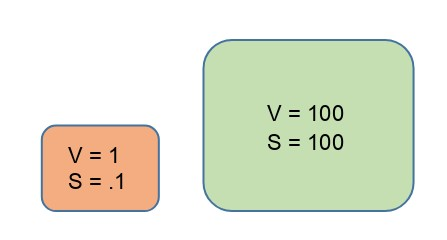
\includegraphics[width=4cm, height=3cm]{knap_greedy.jpg}
\centering
\end{figure}\\
In such a scenario, the smaller box is chosen, when the clear choice is the bigger box.
Although this method is completely useless. The approach maximizes the average density of the occupied space in the knapsack. It doesn't however, account for the empty space. This approach however does work when the objects are small. Say the objects are of size $\frac{1}{k}$ where k large enough. in such a scenario, the maximum empty space is $\frac{1}{k}$ and the approximation ratio can be minimized arbitrarily. So, the greedy approach works for a special case.
\\\\
Now, Let's try to solve the problem for another special case. This time, we assume that the item values are small integers, say less than k.
\[V_i \in \{1, 2,\ldots, k\}\]
in such a scenario, though it is not obvious, there is a Dynamic Programming algorithm that computes the optimal solution. \\
we keep track of a 2D matrix $M$ in which $M[i][V]$ the size of the minimal subset of the first i items that has sum of values = V. \\ 
Now, we can build a recursive algorithm to fill the matrix M.
\begin{figure}[h]
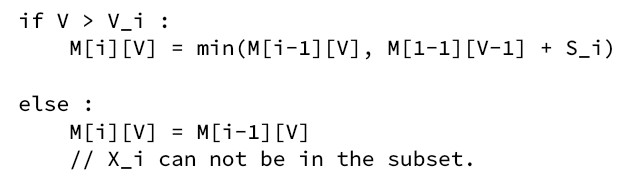
\includegraphics[width=10cm, height=3cm]{knap_rec.jpg}
\centering
\end{figure}\\
Note that for every n this has to go over every value from 0 to $nk$. Making the run time $O(n^2k)$.

So far, we have found an optimal algorithm for the special case where the value is restricted to a small integer. But wht about the case of other values of V ?\\
This is where Rounding comes in. The idea is simple, it seems almost too simple to work. We simply scale down the $V_i$ by dividing them by $max(V_i)/k$, and then round it down to the nearest Integer $V'_i$.\\
Let's see how well this works :\\
\textbf{Analysis :} Let k be $\alpha \cdot n$.(It will soon be clear why such a value is chosen)
Let $Gain$ denote the sum of values of the items returned by the algorithm.
\begin{align*}
Gain &= \sum V'_i \\
	&\geq \sum (\alpha V_i - 1) \\
	&\geq \frac{1}{\alpha}\sum \alpha(V_i - n) \\
	&\geq OPT - \frac{n}{\alpha} 
\end{align*}
Now, we can reasonably assume that $OPT \geq max(V_i)$ 
\begin{align*}
\Rightarrow Gain &\geq \frac{n}{k}OPT \\
	&\geq  OPT (1-\frac{1}{k})
\end{align*}
Now we see why k was chosen to be $\alpha n$. Here we can get an answer to arbitrary precision if we choose a large enough k.
\\
We have successfully helped our friend, the burglar. In the next problem we will use Rounding with Linear programming, in a clever manner.

\subsection*{The diligent Burglar}
Having learned his lesson from the previous incident, out friend the burglar is more diligent this time, and carefully surveys his next target. He now knows the exact sizes$(S_i)$ of the items he has to loot, and intends to loot all the items. He now asks you how many(minimum) knapsacks he must take to to bring home all the items.

Again, we start by defining a mathematical formulation for the problem.

We solve a simpler case of the problem. Assume that all items are large. i.e all $S_i \geq N\cdot \epsilon$. Now, we have a glimpse of hope. The original problem can be reduced to the simpler case, however, this has little to do with approximation algorithms, and is herefore left out of the book.\\ 
Notice that rounding the sizes of the items will only leave us with a constant number of choices(not dependent on the number of items) for the combination of items that can be contained in a knapsack. We can simply exhaustively search all combinations of knapsacks and find the best combination. It gives us the linear program :
\begin{align*}
&find \quad min(\sum x_c) \\
&given \quad \sum a_{s,c} \cdot x_c \geq n_s
\end{align*}
Here $a_{s,c}$ is the number of times an item of size s is in a knapsack of configuration c.\\
Though this seems like a good LP Relaxation, this is not good enough. In a situation where all items have the size $N/3$ or $2N/3$, and there are $n/2$ items of each type, it is apparent that the optimal case is when $n/2$ knapsacks are needed. However, our solution rounds these values to $N/3+0.66$ and $2N/3 + 0.33$, and ends up putting the items of the second type together and the items of the first type in one sack, taking $3n/4$ knapsacks. This is a bad approximation.\\\\
We either have to discard this solution all together of come up with a better way to round the inputs. Turns out, such a rounding exists.
\begin{figure}[h]
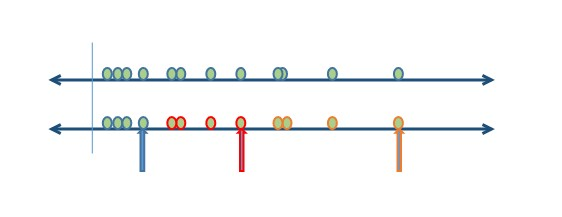
\includegraphics[width=13cm, height=4cm]{binpac.jpg}
\centering
\end{figure}\\
As shown in the above diagram, the items are sorted, divided into groups of $n\epsilon^2$ and rounded to the value of the largest item in the group.\\\\\\\\\\

\textbf{Analysis :}
Let the output be $Y$ \\
Note that in bin packing, the OPT value increases when you increase the input size(round up) and decreases when you decrease the input size(round down).
Now consider a scenario where we round down to the largest element of the previous group. Note that the resultant groups formed are almost identical to that in the case of rounding up. The only major difference is the smallest group in the rounding up and the largest group in the rounding down. The smallest group is rounded to 0 and can be ignored.\\
Let the solution given by this rounding be Z.\\
\begin{align*}
Y &\geq Z + n\epsilon ^2 \\
\therefore  Y &\geq OPT + n\epsilon ^2 \\
\therefore  Y &\geq OPT + \epsilon \cdot OPT \\
\end{align*} \\
We have reached the result that our algorithm give us a solution that is near optimal in polynomial time. \\\\

This Problem demonstrates that rounding often requires considerable amount of thought, and is not always as simple as flooring or ceiling the input. \\
In the next chapter we will look at a different property of linear optimization, and build a heuristic for designing algorithms around it.

 

%%%%%%%%%%%%%%%%%%%%%%%%%%%%%%%%%%%%%%%%%%%%%%%%%%%%%%%%%%%%%%%%%%%%%%%%%%%%%%%%%%%%%%%%%%%

\chapter{Prime-Dual Schema}
So far, we have seen a way to use linear programs to get approximate solutions to Integer Programs. However, rounding is not the only way to accomplish this. Before we get into the other ways to do this, let us first understand the concept of duality.\\
Consider the following LP :\\
Find \begin{equation*}
OPT = min(3x_1 + x_2 + 5x_3)
\end{equation*}
Given :
\begin{align*}
&2x_1 - x_2 + 2x_x \geq 10 \\
&x_1 + x_2 + 2x_3 \geq 7 \\
&x_i \in Z^+
\end{align*} 
Without using any computational trickery, we can tell that $OPT \geq 10$. How ?
\begin{align*}
&\quad\quad\quad\quad\quad\quad\quad\quad x_i \geq 0 \\
&\Rightarrow 3x_1 \geq 2x_1 \quad \& \quad x_2 \geq -x_2 \quad \& \quad 5x_3 \geq 2x_3 \\
&\Rightarrow 3x_1 + x_2 + 5x_3 \geq 2x_1 - x_2 + 2x_3 \\
&\Rightarrow 3x_1 + x_2 + 5x_3 \geq 10
\end{align*}
We can go a step further and say :
\begin{align*}
&\Rightarrow 3x_1 + x_2 + 5x_3 \geq 3x_1 + 4x_3 \\
&\Rightarrow 3x_1 + x_2 + 5x_3 \geq (2x_1 - x_2 + 2x_3) + (x_1 + x_2 + 2x_3)\\
&\Rightarrow 3x_1 + x_2 + 5x_3 \geq 17
\end{align*}
There is no reason why we should restrict ourselves to a simple sum of the 2 equations.
\begin{align*}
if \quad &2y_1 + y_2 \leq 3 \quad \& \\
&-y_1 + y_2 \leq 1 \quad \& \\
&2y_1 + 2y_2 \leq 5 
\end{align*}\begin{align*}
& 3x_1 + x_2 + 5x_3 \geq y_1(2x_1 - x_2 + 2x_3) + y_2(x_1 + x_2 + 2x_3)\\
&\Rightarrow 3x_1 + x_2 + 5x_3 \geq 10y_1 + 7y_2
\end{align*}
Notice that this is another LP(Let's call it D) that maximizes $10y_1 + 7y_2$ under the aforementioned constraints. Solving the 2nd LP for the values $max(10y_1 + 7y_2)$ is equivalent to solving the first LP.\\

We say that D is the dual of P.\\
Since D is also a LP, D also has a dual. Turns out
\[dual(dual(P)) = P\]
this will become more apparent when we represent the equations in the Matrix form.
\begin{align*}
& min(\alpha \cdot A) \quad \quad \quad &max(\beta \cdot B) \\
& Ax \geq \beta                       & By \leq \alpha \\
& x \geq 0							 & y \geq 0	
\end{align*}

Now that we have an understanding of what duality is, with the help of some examples, we will see how to use this to construct approximation algorithms.
\pagebreak

\subsection*{Steiner Forest Problems} 
The input is a weighted undirected graph, with subsets of the vertex set marked as terminals. $T \subset P(V)$ s.t. every pair of sets in $T$ are disjoint. This can be seen as a colouring of G, where all the elements in $T_i$ are of the same colour. Not all elements are coloured. Our goal is  to find the least subgraph that connects all vertices of the same colour.\\\\
\textbf{Steiner Tree Problem :}\\
As usual, we start with a simpler case of the problem. One where there is only one set in T. 
\begin{figure}[h]
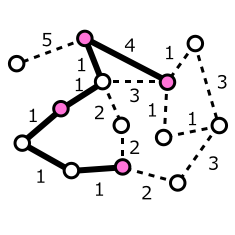
\includegraphics[width=4cm, height=4cm]{steiner_tree.jpg}
\centering
\end{figure}\\
You may have notices that this problem is very similar to the MST problem, which can be easily solved in polynomial time, by say the kruskal's algorithm. And so, we use this knowledge to convert the given problem to a MST problem.\\
Here's a simple algorithm for that :
\begin{figure}[h]
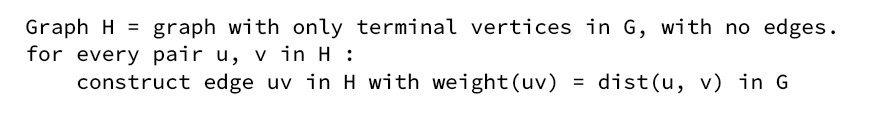
\includegraphics[width=12cm, height=2cm]{stt_algo.jpg}
\centering
\end{figure}\\
Now find a MST on this graph, then, replace the edges in H with their corresponding edges in G. This Algorithm gives an approximate solution within a factor of 2. \\

Back to \textbf{steiner forest}. \\
Now that we have a solution to a simpler problem, let's see if this helps us in any way. 
We can start by constructing our usual Integer Program for the problem.
Let $X_e$ denote whether or not an edge is in the selected solution.\\
Our goal is the following :
\begin{align*}
min(\sum _e w_e \cdot x_e)
\end{align*}
constraint : for every u, v in $T_i$ we want u and v to be connected. We define that as follows : \\
\begin{align*}
\sum _{e\in \delta(x)}x_e  & \geq 1 \quad \forall S \in S^{*} \\
x_e & \in \{0, 1\} 
\end{align*}
Here, S is a set such that it contains either u or v, $S^*$ is the set of all such S. \\
$\delta(S)$ is the set of cross edges form S. \\
At the first glance, this seems to be an integer program like the ones we have solved using LP-relaxations. However, notice that there are a exponential number of equations here, and hence, he LP relaxation can not be solved in polynomial time.

So, we try this with our newly acquired tool, duality.
The dual of the LP is :
\begin{align*}
&min(\sum _s y_s) \\
& \sum _{S:e\in\delta(s)} \leq w_e \\
& y_e \geq 0
\end{align*}
The diagram below shows the intuitive meaning of x and y.
\begin{figure}[h]
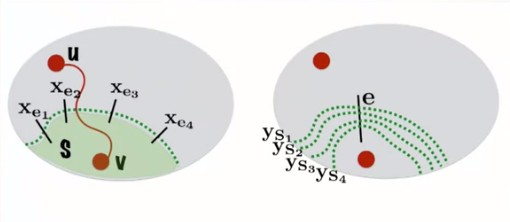
\includegraphics[width=9cm, height=4cm]{cuts.jpg}
\centering
\end{figure}\\


\begin{enumerate}
  \item Initially, we start with all variables at 0. D is feasible, but not P.
  \item Start increasing y (any y) until some constraint e becomes tight. When this 					happens, set $X_e = 1$. Repeat this step till x is feasible.
  \item Raise all $y_s$ that correspond to single unconnected graphs simultaneously by 				small values, until some constraint e becomes tight. When this happens, set$X_e=1$.
  		\\Note that once this is done, there exists an edge e between 2 vertices, say u, v.
  		\\This subgraph $S_i = \{u, v, uv\}$ can now be treated as a singleton graph. 				Hence, we repeat step 3 for the cut $y_{S_i}$ corresponding to this set. 
  \item Stop when all constraints on y are tight.
  \item While this does guarantee a feasible solution, the solutions not the best we can get. There are some redundant edges. However, this problem can be dealt with by simply going through the selected edges and removing the unnecessary edges.
\end{enumerate}

This Algorithm gives a solution that Approximates within a constant factor of OPT.\\\\


The above solution demonstrates the general method of using the prime-dual schema to solve approximate Integer Program solutions :
\begin{enumerate}
  \item Start with a trivial feasible 
  \item Adjust the dual until tight constraints are met. 
  		Repeat this until constraints are tight.
\end{enumerate}

%%%%%%%%%%%%%%%%%%%%%%%%%%%%%%%%%%%%%%%%%%%%%%%%%%%%%%%%%%%%%%%%%%%%%%%%%%%%%%%%%%%%%%%%%%%
\chapter{Semi-Definite Programming}



%%%%%%%%%%%%%%%%%%%%%%%%%%%%%%%%%%%%%%%%%%%%%%%%%%%%%%%%%%%%%%%%%%%%%%%%%%%%%%%%%%%%%%%%%%%
.
\end{document}